\documentclass[amsmath,amssymb,notitlepage,12pt]{revtex4-1}
\usepackage{graphicx}
\usepackage{bm}% bold math
\usepackage{multirow}
\usepackage{booktabs}
\usepackage{verbatim}
\usepackage{hyperref}
\hypersetup{pdftex,colorlinks=true,allcolors=blue}
\usepackage{hypcap}
%\usepackage[small,compact]{titlesec}
%\usepackage{showkeys}
%\addtolength{\textheight}{0.3cm}
%\addtolength{\topmargin}{-0.15cm}
%\addtolength{\textwidth}{0.4cm}
%\addtolength{\hoffset}{-0.2cm}
\begin{document}
%\hspace*{11.5cm}\texttt{HPS-NOTE 2015-XXX}

\title{HPS Chicane Operations Manual v0.1}
\author{N. Baltzell}
\affiliation{Jefferson Lab}
\date{\today}
\begin{abstract}
Controls of the HPS chicane are updated for 2016 to simplify operations during shift.  This includes a simplified user interface, automatic retrieval of beam energy, and automatic calculations of magnet current setpoints.  This manual explains the operations of the new interface. 
\end{abstract}
\maketitle

\section{New GUI}

As far as manipulating the magnets' power supplies, this new user interface only sets the current setpoints, but in an automated way based on beam energy and for both Frascati and Pair Spectrometer magnets' power supplies simultaneously.  The primary intent is to minimize the user interaction necessary for energization of the chicane magnets and corresponding dead time.

\begin{figure}[htbp]\centering
    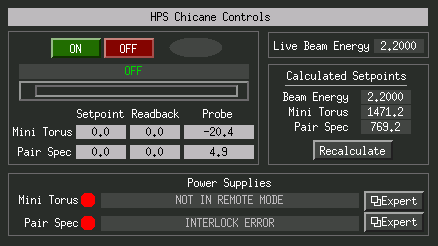
\includegraphics[width=14cm]{pics/gui}
    \caption{The new chicane screen with both magnets power supplies completely off and interlocked, and setpoints calculated for a beam energy of 2.2 GeV.\label{fig:guiChicaneOff}}
\end{figure}

There are 5 buttons for user interaction, and only ``On'' and ``Off'' should be necessary for shift workers:
\begin{itemize}
    \item On
    \item Off
    \item Recalculate
    \item Expert (2)
\end{itemize}

Theses buttons functions are explained in the following sections.

\section{On}
``On'' will perform the procedure to go from chicane off to beam ready.  This would normally be done during operations when preparing for first beam after an extended down time or any time the chicane was turned off.
\begin{enumerate}
    \item ramp both magnets' power supplies up to their max current
    \item sit at max current for N minutes
    \item ramp both magnet power supplies down from their max currents to their setpoints corresponding to expected beam energy.
    \item ready
\end{enumerate}

\section{Off}
``Off'' will just make the setpoint current zero for both magnets, thereby initiating a rampdown.  This would normally be done any time the magnets need to be set to zero.

\section{Recalculate}
``Recalculate'' reads the current Hall-B beam energy from the accelerator and calculates the corresponding setpoints for the HPS chicane magnets:
\begin{enumerate}
    \item reads the current ``Live Beam Energy''
    \item stores it as the setpoint energy
    \item calculates the corresponding magent power supply current setpoints
\end{enumerate}

\section{Expert}
The two ``Expert'' buttons just open the old screens for the two magents power supplies.






\end{document}

